\section{Rancangan Solusi}

\subsection{Arsitektur Sistem}\label{rancangan-solusi-arsitektur-sistem}

Gambaran high-level:
\begin{itemize}
	\item Patient device (Android)
	\item Optional: wearable $\rightarrow$ Android
	\item Local DB + batching engine
	\item Encryption module
	\item IPFS cluster
	\item IOTA node + smart contract DecMed (extended)
	\item Existing DecMed components (proxy, CapBAC, PRE) di mana PGHD diintegrasikan
\end{itemize}



Interval pengambilan data dilakukan setiap interval waktu pada tabel~\ref{health-connect-get-data-interval} \parencite{android_hc_write}.

\begin{table}[htbp]
	\centering
	\caption{Panduan Interval Pengambilan Data}\label{health-connect-get-data-interval}
	\renewcommand{\arraystretch}{1.25}
	\setlength{\tabcolsep}{8pt}
	\rowcolors{2}{white}{white}
	\begin{tabularx}{\textwidth}{>{\raggedright\arraybackslash}p{0.30\textwidth}>{\raggedright\arraybackslash}X}
		\rowcolor[HTML]{DDEBF7}
		\textbf{Tipe Data} & \textbf{Ekspektasi (Frekuensi Penulisan)} \\
		\midrule
		Steps & Setiap 1 menit \\
		\midrule
		StepsCadence & Setiap 1 menit \\
		\midrule
		WheelchairPushes & Setiap 1 menit \\
		\midrule
		ActiveCaloriesBurned & Setiap 15 menit \\
		\midrule
		TotalCaloriesBurned & Setiap 15 menit \\
		\midrule
		Distance & Setiap 1 menit \\
		\midrule
		ElevationGained & Setiap 1 menit \\
		\midrule
		FloorsClimbed & Setiap 1 menit \\
		\midrule
		HeartRate & 4 kali per menit \\
		\midrule
		HeartRateVariabilityRmssd & Setiap 1 menit \\
		\midrule
		RespiratoryRate & Setiap 1 menit \\
		\midrule
		OxygenSaturation & Setiap jam \\
		\bottomrule
	\end{tabularx}
\end{table}



Interval 15 menit dipilih merujuk pada panduan penulisan data Health Connect API yang merekomendasikan interval tersebut untuk tipe data fisiologis
Durasi yang digunakan untuk mengirimkan data dari klien ke sistem DecMed adalah setiap 15 menit sekali seperti rekomendasi Google HealthConnect API \parencite{android_hc_write}.

\subsection{Mekanisme Verifikasi Kerahasiaan, Integritas dan Ketersediaan PGHD}\label{rancangan-mekanisme-integritas-nonrepudiation}

Berdasarkan pemilihan pada subbab~\ref{alternatif-analisis-solusi-cia}, diperlukan suatu mekanisme untuk memverifikasi kerahasiaan, integritas, dan ketersediaan data PGHD\@.
Mekanisme yang dipilih untuk menjamin kerahasiaan adalah mekanisme enkripsi data PGHD, sementara mekanisme untuk menjamin integritas adalah kombinasi hash dengan digital signature, dan mekanisme untuk menjamin ketersediaan adalah mekanisme \textit{batching} dan penyimpanan data PGHD di IPFS, bukan di \textit{on-chain} IOTA\@.
Sama seperti rekam medis elektronik yang dihasilkan oleh tenaga kesehatan, data PGHD yang dihasilkan pasien akan disimpan di IPFS, sementara metadata dan informasi mengenai data akan disimpan di \textit{on-chain} IOTA mempertimbangkan keterbatasan IOTA untuk menyimpan data maksimum berukuran 250 KB\@.
Selain itu, sejalan dengan strategi pengiriman dan penyimpanan data pada alternatif \textit{pipeline} di subbab~\ref{alternatif-arsitektur-pipeline-pghd} dan arsitektur \textit{pipeline} di subbab~\ref{rancangan-solusi-arsitektur-sistem}, akan digunakan mekanisme \textit{batching} sehingga jaringan dan sistem DecMed tidak \textit{overload} terhadap transaksi yang sedang berjalan.

Untuk menjamin kerahasiaan PGHD, klien pasien melakukan enkripsi data PGHD sebelum dikirim ke DecMed dan disimpan di IPFS\@.
Hal ini dilakukan agar data PGHD tidak dapat diakses oleh orang yang tidak memiliki hak akses baik ketika data dikirim ataupun sudah disimpan di IPFS DecMed\@.

Untuk menjamin integritas PGHD, klien pasien menghitung hash dari PGHD sebelum data dienkripsi.
Kemudian hash tersebut ditandatangani oleh kunci privat pasien menjadi digital signature.
Kedua data tersebut dikirim ke DecMed, di mana PGHD yang dienkripsi akan disimpan di IPFS, dan smart contract akan memverifikasi digital signature menggunakan kunci publik pasien.
Jika digital signature valid, maka hal ini berarti nilai hash tidak dimodifikasi. 

Smart contract kemudian akan melakukan dekripsi digital signature dan didapatkan hash yang dikirim dari klien pasien.
Untuk memverifikasi apakah data PGHD yang disimpan di IPFS valid atau tidak, smart contract perlu menghitung ulang hash dari data yang dikirim.
Namun karena baik smart contract, PRE maupun IPFS tidak dapat mendekripsi data PGHD sama sekali dan smart contract tidak dapat mengolah data berukuran di atas 250 KB, maka dekripsi dan penghitungan hash PGHD tidak dapat dilakukan dalam sistem DecMed.
Sistem DecMed menjamin keamanan data pasien dengan mekanisme proxy-reencryption sehingga pasien tidak perlu mengirimkan kunci privatnya untuk tenaga kesehatan dapat mengakses rekam medisnya.
Proxy reencryption bekerja dengan \dots (referensi PRE, jelaskan PRE secara singkat, tambah subbab PRE di studi literatur/dasar teori).
Hal ini membuat DecMed tidak memungkinkan untuk melakukan dekripsi 

Untuk mengatasi hal tersebut, dibuat mekanisme digital signature rangkap (bawa penjelasan di rancangan fungsionalitas).



Struktur metadata yang disimpan secara \textit{on-chain} pada ledger IOTA untuk setiap entri PGHD dirancang sebagai berikut:
\begin{itemize}
    \item \verb|patient_id|: alamat IOTA pasien (\verb|iota_address|) sebagai identitas kriptografis yang unik,
    \item \verb|cid|: \textit{Content Identifier} IPFS yang merujuk ke \textit{payload} PGHD terenkripsi (\verb|enc_pghd|),
    \item \verb|enc_aes_key_nonce|: ciphertext yang berisi gabungan kunci AES dan \textit{nonce} yang telah dienkripsi menggunakan \verb|pre_public_key| pasien melalui mekanisme proxy re-encryption,
    \item \verb|capsule|: artefak kriptografis proxy re-encryption yang diperlukan untuk merekonstruksi kunci AES di sisi klien yang berhak,
    \item \verb|pghd_outer_signature|: \textit{digital signature} yang dihasilkan dari penandatanganan nilai hash SHA-256 dari \verb|enc_pghd| menggunakan kunci privat pasien \verb|pghd_secret_key|,
    \item \verb|h_cipher|: nilai hash SHA-256 dari ciphertext \verb|enc_pghd| yang dihitung oleh klien pasien,
    \item \verb|status|: status entri PGHD (\texttt{VALID} atau \texttt{INVALID}) yang digunakan untuk menandai apakah entri masih dapat digunakan oleh aplikasi,
    \item \verb|timestamp|: waktu pencatatan data ke dalam sistem.
\end{itemize}

(Di sini kita juga perlu menjelaskan mengenai strategi pengaksesan data saat kondisi gawat darurat, rawat jalan, rawat inap, dll seperti dijelaskan di subbab~\ref{alternatif-arsitektur-pipeline-pghd}).

\subsection{Rancangan Format dan Skema PGHD}\label{rancangan-format-data-pghd}

Berdasarkan pemilihan solusi pada Subbab~\ref{alternatif-provenance} dan landasan teori pada Subbab~\ref{studi-cia-provenance}, bagian ini merancang format data yang digunakan PGHD untuk mendukung \textit{data provenance}.
\textit{Payload} PGHD yang disimpan di penyimpanan \textit{off-chain} terdiri atas tingkat \textit{batch}, tingkat \textit{data group}, dan tingkat \textit{data point}.
Tingkat \textit{batch} merepresentasikan satu paket pengiriman PGHD\@.
Tingkat \textit{data group} mengelompokkan data berdasarkan jenis pengukuran dan sumber data.
Tingkat \textit{data point} merepresentasikan nilai pengukuran individual.
Tabel~\ref{tab:field-batch-json-pghd} menjelaskan \textit{fields} pada tingkat \textit{batch}.

\begingroup
\footnotesize
\begin{styledxltabular}{|>{\raggedright\arraybackslash}p{0.22\textwidth}|>{\raggedright\arraybackslash}p{0.15\textwidth}|>{\raggedright\arraybackslash}p{0.12\textwidth}|>{\raggedright\arraybackslash}X|}
    \hiderowcolors
    \caption{Deskripsi \textit{Field} Tingkat \textit{Batch} pada Skema JSON untuk PGHD}\label{tab:field-batch-json-pghd}\\
    \hline
    \rowcolor{headerBg}
    \textbf{Field} & \textbf{Tipe} & \textbf{Wajib} & \textbf{Deskripsi} \\
    \hline
    \showrowcolors
    \endfirsthead

    \hiderowcolors
    \caption[]{Deskripsi \textit{Field} Tingkat \textit{Batch} pada Skema JSON untuk PGHD (lanjutan)}\\
    \hline
    \rowcolor{headerBg}
    \textbf{Field} & \textbf{Tipe} & \textbf{Wajib} & \textbf{Deskripsi} \\
    \hline
    \showrowcolors
    \endhead

    \texttt{schema\_version} & String & Ya & Versi skema JSON PGHD yang digunakan. \\
    \hline
    \texttt{batch\_id} & UUID & Ya & Identitas unik \textit{batch}. \\
    \hline
    \texttt{patient\_id} & String & Ya & Identitas pasien pada sistem DecMed, diisi dengan alamat IOTA akun pasien. \\
    \hline
    \texttt{source\_device} & Objek & Ya & Metadata perangkat pengirim \textit{batch}, meliputi \texttt{type}, \texttt{platform}, \texttt{app\_version}, \texttt{device\_manufacturer}, dan \texttt{device\_model}. \\
    \hline
    \texttt{batch\_period} & Objek & Ya & Rentang waktu yang dicakup oleh \textit{batch}, terdiri atas \texttt{start\_timestamp} dan \texttt{end\_timestamp} dalam format Unix \textit{timestamp}. \\
    \hline
    \texttt{trigger\_reason} & String & Tidak & Alasan pembentukan atau pengiriman \textit{batch}, misalnya pengiriman periodik, ambang ukuran data, pengiriman manual, atau koneksi tersedia kembali. \\
    \hline
    \texttt{data\_group} & Array & Ya & Daftar grup data PGHD yang dijelaskan pada Tabel~\ref{tab:field-datagroup-json-pghd}. \\
    \hline
\end{styledxltabular}
\endgroup

% Implementasi Android saat ini menggunakan nilai trigger time_based, size_threshold, manual_submit, dan network_available.

Sebuah \textit{batch} terdiri dari kumpulan \texttt{data\_group}.
Setiap elemen di dalam \texttt{data\_group} mengelompokkan data berdasarkan tipe pengukuran dan asal data.
Tabel~\ref{tab:field-datagroup-json-pghd} menjelaskan \textit{fields} pada tingkat \textit{data group}.

\begingroup
\footnotesize
\begin{styledxltabular}{|>{\raggedright\arraybackslash}p{0.25\textwidth}|>{\raggedright\arraybackslash}p{0.15\textwidth}|>{\raggedright\arraybackslash}p{0.12\textwidth}|>{\raggedright\arraybackslash}X|}
    \hiderowcolors
    \caption{Deskripsi \textit{Field} Tingkat \textit{Data Group} pada Skema JSON untuk PGHD}\label{tab:field-datagroup-json-pghd}\\
    \hline
    \rowcolor{headerBg}
    \textbf{Field} & \textbf{Tipe} & \textbf{Wajib} & \textbf{Deskripsi} \\
    \hline
    \showrowcolors
    \endfirsthead

    \hiderowcolors
    \caption[]{Deskripsi \textit{field} tingkat \textit{data group} pada skema JSON untuk PGHD (lanjutan)}\\
    \hline
    \rowcolor{headerBg}
    \textbf{Field} & \textbf{Tipe} & \textbf{Wajib} & \textbf{Deskripsi} \\
    \hline
    \showrowcolors
    \endhead

    \texttt{measurement\_type} & String & Ya & Jenis pengukuran dalam format \textit{snake\_case}, misalnya \texttt{heart\_rate}, \texttt{steps}, atau tipe pengukuran kesehatan lain yang didukung sistem. \\
    \hline
    \texttt{device\_type} & String & Ya & Tipe perangkat atau sumber penghasil pengukuran, misalnya \textit{mobile}, perangkat \textit{wearable}, atau input manual. \\
    \hline
    \texttt{recording\_method} & String & Tidak & Cara data direkam, misalnya otomatis oleh perangkat, sesi aktif, input manual, atau hasil transformasi dari data sensor. \\
    \hline
    \texttt{source} & String & Ya & Kategori sumber data, misalnya API OS untuk wellness/fitness/activity, sensor perangkat, atau input manual. \\
    \hline
    \texttt{source\_label} & String & Tidak & Label sumber yang lebih mudah dibaca pengguna atau tenaga kesehatan. \\
    \hline
    \texttt{source\_package\_name} & String & Tidak & Identitas aplikasi atau paket sumber data apabila tersedia dari API OS\@. \\
    \hline
    \texttt{device\_source} & String & Tidak & Informasi sumber perangkat atau metode derivasi, misalnya perangkat wearable, sensor telepon, atau data dari sensor yang sudah diolah. \\
    \hline
    \texttt{statistics} & Array & Ya & Ringkasan statistik per \textit{field} numerik yang terdiri atas jumlah data, minimum, maksimum, rata-rata, median, modus, dan persentil. Struktur elemen dijelaskan pada Tabel~\ref{tab:field-statistics-json-pghd}. \\
    \hline
    \texttt{clinical\_thresholds} & Array & Ya & Salinan rentang klinis yang dipakai klien pasien saat membentuk \textit{batch}, termasuk satuan, konteks populasi, nama referensi, dan URL referensi. Tipe data tanpa rentang klinis umum menggunakan array kosong. \\
    \hline
    \texttt{anomaly\_count} & Integer & Ya & Jumlah seluruh penanda anomali pada \textit{data group}. \\
    \hline
    \texttt{data\_points} & Array & Ya & Daftar nilai pengukuran aktual yang dijelaskan pada Tabel~\ref{tab:field-datapoints-json-pghd}. \\
    \hline
\end{styledxltabular}
\endgroup

% Implementasi Android saat ini menggunakan label sumber Health Connect, Phone Sensor, dan Manual Input. Nama API spesifik tersebut dijelaskan pada Bab IV.

\textit{Data group} berisi kumpulan \textit{data points} individual yang merupakan hasil pengukuran untuk setiap satuan waktu atau setiap periode pengukuran.
Tabel~\ref{tab:field-datapoints-json-pghd} berisi skema data untuk level \textit{data points}.

\begingroup
\footnotesize
\begin{styledxltabular}{|>{\raggedright\arraybackslash}p{0.22\textwidth}|>{\raggedright\arraybackslash}p{0.15\textwidth}|>{\raggedright\arraybackslash}p{0.12\textwidth}|>{\raggedright\arraybackslash}X|}
    \hiderowcolors
    \caption{Deskripsi \textit{Field} Tingkat \textit{Data Points} pada Skema JSON untuk PGHD}\label{tab:field-datapoints-json-pghd}\\
    \hline
    \rowcolor{headerBg}
    \textbf{Field} & \textbf{Tipe} & \textbf{Wajib} & \textbf{Deskripsi} \\
    \hline
    \showrowcolors
    \endfirsthead

    \hiderowcolors
    \caption[]{Deskripsi \textit{field} tingkat \textit{data points} pada skema JSON untuk PGHD (lanjutan)}\\
    \hline
    \rowcolor{headerBg}
    \textbf{Field} & \textbf{Tipe} & \textbf{Wajib} & \textbf{Deskripsi} \\
    \hline
    \showrowcolors
    \endhead

    \texttt{timestamp} & Unix timestamp & Ya & Waktu pengukuran atau waktu akhir periode pengukuran. \\
    \hline
    \texttt{value} & Number / Objek & Ya & Nilai pengukuran. Untuk pengukuran skalar diisi sebagai bilangan. Untuk pengukuran komposit diisi sebagai objek. \\
    \hline
    \texttt{unit} & String & Ya & Satuan pengukuran. \\
    \hline
    \texttt{anomalies} & Array & Ya & Daftar penanda untuk setiap \textit{field} yang berada di bawah atau di atas rentang klinis. Array kosong menandakan tidak ada anomali yang ditemukan atau tipe data tidak memiliki rentang umum yang dikonfigurasi. \\
    \hline
\end{styledxltabular}
\endgroup

\begingroup
\footnotesize
\begin{styledxltabular}{|>{\raggedright\arraybackslash}p{0.23\textwidth}|>{\raggedright\arraybackslash}p{0.18\textwidth}|>{\raggedright\arraybackslash}X|}
    \hiderowcolors
    \caption{Struktur Elemen \texttt{statistics} PGHD}\label{tab:field-statistics-json-pghd}\\
    \hline
    \rowcolor{headerBg}
    \textbf{Field} & \textbf{Tipe} & \textbf{Deskripsi} \\
    \hline
    \showrowcolors
    \endfirsthead
    \hline
    \rowcolor{headerBg}
    \textbf{Field} & \textbf{Tipe} & \textbf{Deskripsi} \\
    \hline
    \endhead
    \texttt{field} & String & Nama komponen numerik yang diringkas. \\
    \hline
    \texttt{count} & Integer & Jumlah nilai numerik. \\
    \hline
    \texttt{minimum}, \texttt{maximum} & Number & Nilai terkecil dan terbesar. \\
    \hline
    \texttt{mean}, \texttt{median} & Number & Nilai rata-rata dan median. \\
    \hline
    \texttt{mode} & Array Number & Seluruh nilai dengan frekuensi tertinggi; kosong apabila tidak ada nilai berulang. \\
    \hline
    \texttt{percentiles} & Objek & Nilai \texttt{p5}, \texttt{p25}, \texttt{p50}, \texttt{p75}, dan \texttt{p95}. \\
    \hline
    \texttt{unit} & String & Satuan statistik. \\
    \hline
\end{styledxltabular}
\endgroup

\begingroup
\footnotesize
\begin{styledxltabular}{|>{\raggedright\arraybackslash}p{0.25\textwidth}|>{\raggedright\arraybackslash}p{0.17\textwidth}|>{\raggedright\arraybackslash}X|}
    \hiderowcolors
    \caption{Struktur Rentang Klinis dan Penanda Anomali PGHD}\label{tab:field-threshold-anomaly-json-pghd}\\
    \hline
    \rowcolor{headerBg}
    \textbf{Struktur/Field} & \textbf{Tipe} & \textbf{Deskripsi} \\
    \hline
    \showrowcolors
    \endfirsthead
    \hline
    \rowcolor{headerBg}
    \textbf{Struktur/Field} & \textbf{Tipe} & \textbf{Deskripsi} \\
    \hline
    \endhead
    \texttt{clinical\_\allowbreak{}thresholds.\allowbreak{}field} & String & \textit{Field} numerik yang dievaluasi. \\
    \hline
    \texttt{minimum}, \texttt{maximum} & Number & Batas bawah dan atas rentang. \\
    \hline
    \texttt{minimum\_inclusive}, \texttt{maximum\_inclusive} & Boolean & Menentukan apakah nilai tepat pada batas masih termasuk rentang. \\
    \hline
    \texttt{unit}, \texttt{label}, \texttt{population} & String & Satuan, nama rentang, serta populasi atau konteks penerapan. \\
    \hline
    \texttt{reference}, \texttt{reference\_url} & String & Identitas dan alamat sumber rentang yang ikut dikirim kepada tenaga kesehatan. \\
    \hline
    \texttt{anomalies.field}, \texttt{anomalies.value} & String, Number & Komponen yang menyimpang dan nilai aslinya. \\
    \hline
    \texttt{anomalies.direction} & String & \texttt{below\_range} atau \texttt{above\_range}. \\
    \hline
    \texttt{normal\_minimum}, \texttt{normal\_maximum} & Number & Batas yang menyebabkan penanda tersebut terbentuk. \\
    \hline
\end{styledxltabular}
\endgroup


\subsection{Rancangan Format Data Lokal}\label{rancangan-solusi-format-data-lokal}

Untuk menangani mekanisme \textit{retry mechanism}, klien pasien menyimpan
setiap \textit{batch} PGHD dalam \textit{local database} dengan struktur pada
Tabel~\ref{tab:field-batch-pghd-local}.

\begin{table}[htbp]
    \centering
    \caption{Struktur Data Lokal Batch PGHD}\label{tab:field-batch-pghd-local}
    \begin{styledtable}{>{\raggedright\arraybackslash}p{0.3\textwidth} >{\raggedright\arraybackslash}p{0.18\textwidth} >{\raggedright\arraybackslash}X}
        \textbf{Field} & \textbf{Tipe} & \textbf{Deskripsi} \\
        \texttt{batch\_id} & UUID & Identitas unik batch, sama dengan field pada skema JSON (Tabel~\ref{tab:field-batch-json-pghd}). \\
        \texttt{enc\_pghd} & String (Base64) & Ciphertext hasil enkripsi (AES-GCM) dari payload PGHD\@. \\
        \texttt{enc\_aes\_key\_nonce} & String (Base64) & Kunci AES dan nonce yang dienkripsi untuk kebutuhan PRE nantinya\@. \\
        \texttt{capsule} & String (Base64) & Artefak kriptografis untuk kebutuhan PRE nantinya. \\
        \texttt{h\_cipher} & String (Hex) & Hash SHA-256 dari \texttt{enc\_pghd}. \\
        \texttt{pghd\_outer\_signature} & String (Base64) & Tanda tangan digital dari \texttt{h\_cipher}. \\
        \texttt{status} & Enum & Status pengiriman: \texttt{pending} (belum dikirim), \texttt{sent} (berhasil), \texttt{failed} (gagal sementara), \texttt{permanent\_failure} (gagal permanen). \\
        \texttt{retry\_count} & Integer & Jumlah percobaan pengiriman (default 0, maksimal 3). \\
        \texttt{created\_at} & Timestamp & Waktu batch dibuat (Unix timestamp). \\
        \texttt{last\_attempt} & Timestamp & Waktu percobaan pengiriman terakhir (Unix timestamp). \\
    \end{styledtable}
\end{table}

Sebelum PGHD dibentuk menjadi batch dan dienkripsi untuk dikirimkan ke sistem,
aplikasi pasien menyimpan data PGHD dalam bentuk lokal raw seperti dapat
dilihat pada Tabel~\ref{tab:field-pghd-raw-local}. Data ini digunakan agar
pasien dapat melihat kembali data kesehatannya sendiri, termasuk sumber data
dan status sinkronisasinya.

\begin{table}[H]
    \centering
    \caption{Format Data PGHD Lokal Raw}\label{tab:field-pghd-raw-local}
    \begin{styledtable}{>{\raggedright\arraybackslash}p{0.3\textwidth} >{\raggedright\arraybackslash}p{0.18\textwidth} >{\raggedright\arraybackslash}X}
        \textbf{Field} & \textbf{Tipe} & \textbf{Keterangan} \\
        \texttt{record\_id} & String & Identitas unik data PGHD lokal. \\
        \texttt{patient\_id} & String & Identitas pasien pada aplikasi. \\
        \texttt{type} & String & Jenis data kesehatan, misalnya langkah, detak jantung, atau kalori. \\
        \texttt{value} & Number & Nilai pengukuran. \\
        \texttt{unit} & String & Satuan pengukuran. \\
        \texttt{timestamp} & DateTime & Waktu pengukuran. \\
        \texttt{source} & String & Sumber data, misalnya Health Connect atau sensor perangkat. \\
        \texttt{source\_package} & String & Nama paket aplikasi sumber data apabila berasal dari Health Connect. \\
        \texttt{sync\_status} & Enum & Status sinkronisasi. \\
        \texttt{created\_at} & DateTime & Waktu data disimpan di perangkat. \\
    \end{styledtable}
\end{table}

\subsection{Fungsionalitas Sistem}

Alur sistem DecMed yang akan diintegrasikan dengan PGHD dapat dilihat melalui Gambar~\ref{fig:flow-decmed-pghd}.

\begin{figure}[htbp]
    \centering
	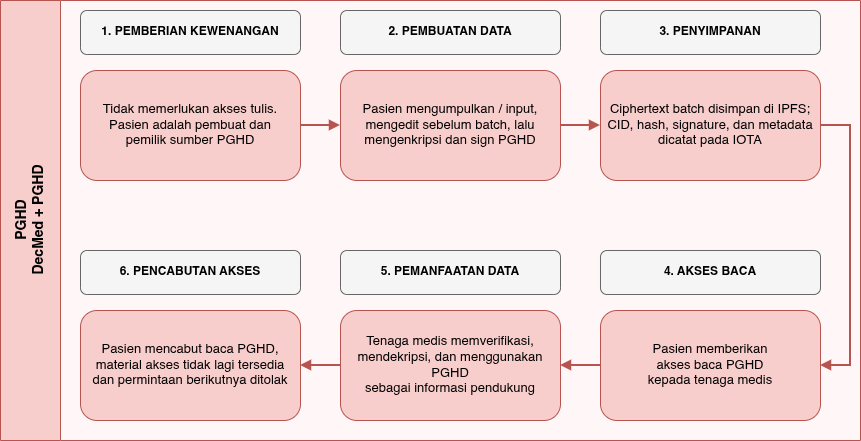
\includegraphics[width=\textwidth]{resources/chapter-3/flow-decmed-pghd.png}
	\caption{Flow Data PGHD di Sistem DecMed-PGHD}\label{fig:flow-decmed-pghd}
\end{figure}

\subsection{Rancangan Register dan Login Pasien PGHD}

Mekanisme register dan login pasien PGHD menggunakan pembangkitan identitas dan kunci kriptografi secara deterministik dari kombinasi \textit{seed words} dan NIK pasien. Pendekatan ini membuat pasien dapat memulihkan identitas yang sama pada proses login ulang selama \textit{seed words}, NIK, dan PIN yang dimasukkan sesuai.

Terdapat tiga komponen kredensial yang memiliki peran berbeda. \textit{Seed words} digunakan sebagai material pemulihan utama untuk membangkitkan ulang identitas dan pasangan kunci pasien. PIN digunakan sebagai faktor lokal untuk membuka atau melindungi material rahasia yang tersimpan pada perangkat, sehingga PIN bukan sumber identitas on-chain, melainkan mekanisme proteksi lokal. CID digunakan setelah PGHD dikirim sebagai rujukan konten terenkripsi pada penyimpanan off-chain. Dengan demikian, CID tidak dibutuhkan untuk melakukan login, tetapi dibutuhkan oleh PRE dan client tenaga kesehatan ketika mengambil, memverifikasi, atau menginvalidasi batch PGHD tertentu.

Pada setiap login, pasien harus menggunakan \textit{seed words}, NIK, dan PIN yang sama agar client dapat membangkitkan alamat IOTA dan kunci kriptografi yang sama. Jika \textit{seed words} atau NIK berbeda, alamat IOTA dan pasangan kunci yang dihasilkan juga berbeda sehingga sistem menganggapnya sebagai identitas lain. Akibatnya, pasien tidak dapat menandatangani transaksi sebagai akun lama, tidak dapat menghasilkan kunci PGHD/PRE yang cocok dengan data lama, dan tenaga kesehatan tidak dapat membuka PGHD lama yang bergantung pada kunci tersebut. Jika PIN berbeda tetapi \textit{seed words} dan NIK benar, kegagalan terutama terjadi pada pembukaan material lokal yang terenkripsi atau tersimpan aman; pasien perlu menggunakan PIN yang sesuai atau melakukan pemulihan ulang sesuai mekanisme aplikasi.

\subsubsection{Variabel yang Dibangkitkan}

Pada proses register maupun login, client pasien membangkitkan beberapa variabel utama sebagai berikut.

\begin{longtable}{|p{0.28\textwidth}|p{0.58\textwidth}|}
    \caption{Variabel identitas dan kriptografi pasien PGHD}
    \label{tab:variabel-register-login-pghd} \\
    \hline
    \textbf{Variabel} & \textbf{Fungsi} \\
    \hline
    \endfirsthead
    \hline
    \textbf{Variabel} & \textbf{Fungsi} \\
    \hline
    \endhead
    \texttt{mnemonic} atau \textit{seed words} & Frasa pemulihan 12 kata yang menjadi sumber pembangkitan identitas pasien. \\
    \hline
    \texttt{patient\_id} dan \texttt{patient\_id\_hash} & Identitas pasien dan bentuk hash dari identitas tersebut yang digunakan untuk pencatatan tanpa membuka NIK mentah. \\
    \hline
    \texttt{iota\_address} & Alamat akun IOTA pasien yang digunakan untuk interaksi dengan smart contract. \\
    \hline
    \texttt{iota\_key\_pair} & Pasangan kunci IOTA pasien untuk menandatangani transaksi dan pesan autentikasi. \\
    \hline
    \texttt{pghd\_public\_key} dan \texttt{pghd\_secret\_key} & Pasangan kunci ECDSA pasien untuk tanda tangan digital data PGHD. \texttt{pghd\_public\_key} disimpan pada smart contract dan digunakan untuk verifikasi tanda tangan. \\
    \hline
    \texttt{pghd\_pre\_public\_key} dan \texttt{pghd\_pre\_secret\_key} & Pasangan kunci PRE khusus PGHD. Kunci ini digunakan dalam enkripsi kunci AES dan mekanisme re-enkripsi akses PGHD. \texttt{pghd\_pre\_public\_key} tidak disimpan sebagai field on-chain PGHD. \\
    \hline
    \texttt{medical\_pre\_public\_key} dan \texttt{medical\_pre\_secret\_key} & Pasangan kunci PRE untuk mekanisme akses rekam medis normal. Kunci ini dipisahkan dari kunci PRE PGHD. \\
    \hline
\end{longtable}

\subsubsection{Alur Register Pasien PGHD}

Alur register pasien PGHD adalah sebagai berikut.

\begin{enumerate}
    \item Pasien membangkitkan atau memasukkan \textit{seed words} sebanyak 12 kata.
    \item Pasien memasukkan NIK dan PIN.
    \item Client membentuk \textit{seed} deterministik dari \textit{seed words} dan NIK.
    \item Client membangkitkan \texttt{iota\_address} dan \texttt{iota\_key\_pair}.
    \item Client membangkitkan \texttt{pghd\_public\_key}, \texttt{pghd\_secret\_key}, \texttt{pghd\_pre\_public\_key}, \texttt{pghd\_pre\_secret\_key}, \texttt{medical\_pre\_public\_key}, dan \texttt{medical\_pre\_secret\_key}.
    \item Client memanggil helper kriptografi untuk melakukan registrasi akun pasien dan publikasi \texttt{pghd\_public\_key} ke smart contract IOTA.
    \item Client mengirimkan registrasi tambahan ke PRE agar PRE dapat melakukan validasi kunci publik PGHD ketika dibutuhkan.
    \item Client menyimpan profil pasien dan kunci terkait ke penyimpanan lokal aman.
    \item Status sesi diubah menjadi \texttt{unlocked} sehingga pasien masuk ke aplikasi.
\end{enumerate}

% Implementasi Android saat ini menggunakan JNI untuk memanggil library Rust serta DataStore/secure storage lokal untuk menyimpan state akun.

\subsubsection{Alur Login Pasien PGHD}

Alur login pasien PGHD adalah sebagai berikut.

\begin{enumerate}
    \item Pasien memasukkan \textit{seed words}, NIK, dan PIN.
    \item Client membangkitkan ulang seluruh identitas dan kunci deterministik dari kombinasi \textit{seed words} dan NIK.
    \item Client memastikan akun pasien telah terdaftar pada smart contract IOTA.
    \item Client melakukan \textit{push registration} ke PRE untuk memastikan PRE memiliki data kunci publik PGHD terbaru.
    \item Client menyimpan kembali profil pasien ke penyimpanan lokal dan mengubah status sesi menjadi \texttt{unlocked}.
\end{enumerate}

Dengan mekanisme ini, kunci pasien tidak dibangkitkan secara acak pada setiap login. Kunci yang sama akan dibentuk ulang dari material pemulihan yang sama. Hal ini penting agar data PGHD lama tetap dapat didekripsi dan diverifikasi selama pasien menggunakan identitas yang sama.


\subsubsection{Mekanisme Pengumpulan PGHD pada Klien Pasien}\label{subsubsec:pengumpulan-pghd}


\subsubsection{Mekanisme Pengiriman PGHD oleh Pasien}\label{subsubsec:pengiriman-pghd}


\begin{enumerate}
    \item \textbf{Pembangkitan kunci penandatanganan PGHD.}
    Pada saat registrasi akun pasien, selain pasangan kunci IOTA (\verb|iota_key_pair|) dan kunci proxy re-encryption (\verb|pre_public_key|) yang telah dibangkitkan oleh DecMed, klien pasien juga membangkitkan sepasang kunci publik dan kunci privat untuk penandatanganan PGHD menggunakan algoritma ECDSA, menghasilkan \verb|pghd_public_key| dan \verb|pghd_secret_key|. 
    ECDSA dipilih karena ukuran kuncinya yang lebih kecil namun menawarkan tingkat keamanan yang ekuivalen dengan RSA, sehingga lebih hemat komputasi untuk perangkat pasien.
    
    \item \textbf{Publikasi kunci publik ke IOTA.}
    Kunci publik \verb|pghd_public_key| dikirim dan disimpan pada ledger IOTA sebagai bagian dari metadata identitas pasien. 
    Dengan demikian, komponen lain di ekosistem DecMed dapat memverifikasi \textit{digital signature} PGHD menggunakan \verb|pghd_public_key| tanpa bergantung pada penyimpanan kunci di sisi klien.
    
    \item \textbf{Pembentukan payload plaintext dan \textit{inner signature}.}
    Ketika data PGHD akan dikirim, klien pasien terlebih dahulu membentuk payload PGHD dalam bentuk plaintext. 
    Klien kemudian menghitung nilai \textit{hash} plaintext dengan fungsi SHA-256,
    \[
        h_{\text{plain}} = \mathrm{SHA256}(\texttt{pghd\_plaintext}),
    \]
    dan menghasilkan \textit{digital signature} \verb|pghd_inner_signature| dengan menandatangani \verb|h_plain| menggunakan \verb|pghd_secret_key| melalui algoritma ECDSA\@. 
    Payload plaintext dan \verb|pghd_inner_signature| kemudian digabungkan ke dalam satu struktur data (field \verb|pghd_data| dan \verb|inner_signature|) sebelum dienkripsi.
    
    \item \textbf{Enkripsi payload PGHD.}
    Struktur data gabungan yang berisi payload PGHD dan \verb|pghd_inner_signature| kemudian dienkripsi menggunakan algoritma AES-GCM dengan kunci simetris acak \verb|aes_key| dan \verb|aes_nonce|, menghasilkan ciphertext \verb|enc_pghd|. 
    Selanjutnya, \verb|aes_key| dan \verb|aes_nonce| digabungkan dan dienkripsi menggunakan \verb|pre_public_key| milik pasien melalui mekanisme proxy re-encryption, menghasilkan pasangan \verb|enc_aes_key_nonce| dan \verb|capsule| serupa dengan mekanisme penambahan rekam medis oleh tenaga kesehatan.
    
    \item \textbf{Pembangkitan \textit{outer digital signature} atas ciphertext.}
    Untuk menjamin integritas dan \textit{non-repudiation} tanpa membebani komputasi \textit{on-chain}, klien pasien menghitung nilai \textit{hash} dari \verb|enc_pghd| (yang dapat berukuran besar) secara lokal di memori klien menggunakan fungsi SHA-256:
    \[
        h_{\text{cipher}} = \mathrm{SHA256}(\texttt{enc\_pghd}).
    \]
    Nilai \verb|h_cipher| kemudian ditandatangani menggunakan kunci privat pasien \verb|pghd_secret_key| dengan algoritma ECDSA, sehingga diperoleh \textit{outer digital signature} \verb|pghd_outer_signature|.
    
    \item \textbf{Pengunggahan off-chain dan pengiriman metadata ke \textit{smart contract}.}
    Klien pasien mengirimkan payload lengkap (\verb|enc_pghd|, \verb|h_cipher|, \verb|enc_aes_key_nonce|, \verb|capsule|, dan \verb|pghd_outer_signature|) ke proxy. 
    Proxy bertindak sebagai perantara \textit{off-chain} dengan mengunggah \verb|enc_pghd| ke kluster IPFS terlebih dahulu untuk mendapatkan \textit{Content Identifier} (CID). 
    Setelah CID diperoleh, proxy memanggil fungsi \texttt{submit\_pghd} pada \textit{smart contract} DecMed. 
    Payload yang dikirimkan ke jaringan IOTA\@: CID, \verb|h_cipher|, \verb|enc_aes_key_nonce|, \verb|capsule|, dan \verb|pghd_outer_signature|.
    
    \item \textbf{Verifikasi \textit{outer digital signature} dan penyimpanan state di IOTA.}
    Setelah menerima pemanggilan fungsi, \textit{smart contract} memproses metadata dengan langkah berikut:
    \begin{enumerate}
        \item memuat \verb|pghd_public_key| pasien dari state \textit{on-chain}, dan
        \item memverifikasi \verb|pghd_outer_signature| terhadap nilai \verb|h_cipher| yang diterima sebagai parameter menggunakan algoritma ECDSA\@.
    \end{enumerate}

    Jika verifikasi gagal, transaksi dibatalkan dan metadata tidak disimpan. Jika verifikasi berhasil, \textit{smart contract} secara permanen menyimpan kaitan antara CID IPFS, \verb|h_cipher|, dan metadata kriptografis lainnya pada ledger IOTA\@. 
    \textit{Smart contract} sama sekali tidak berinteraksi dengan data \verb|enc_pghd|.
\end{enumerate}

\subsection{Rancangan Pemberian Akses PGHD}

Pemberian akses PGHD dilakukan oleh pasien melalui client pasien dengan memindai QR Code milik tenaga kesehatan. QR Code tersebut memuat identitas IOTA tenaga kesehatan dan kunci publik PRE tenaga kesehatan yang dibutuhkan untuk membuat delegasi akses terenkripsi.

\subsubsection{Data Masukan Pemberian Akses}

Data utama yang digunakan pada proses pemberian akses PGHD adalah sebagai berikut.

\begin{longtable}{|p{0.30\textwidth}|p{0.56\textwidth}|}
    \caption{Data masukan mekanisme pemberian akses PGHD}
    \label{tab:data-pemberian-akses-pghd} \\
    \hline
    \textbf{Data} & \textbf{Keterangan} \\
    \hline
    \endfirsthead
    \hline
    \textbf{Data} & \textbf{Keterangan} \\
    \hline
    \endhead
    \texttt{hospital\_personnel\_iota\_address} & Alamat IOTA tenaga kesehatan penerima akses. \\
    \hline
    \texttt{hospital\_personnel\_pre\_public\_key} & Kunci publik PRE tenaga kesehatan yang digunakan untuk mengenkripsi material akses. \\
    \hline
    \texttt{patient\_iota\_address} & Alamat IOTA pasien pemberi akses. \\
    \hline
    \texttt{patient\_iota\_key\_pair} & Kunci IOTA pasien untuk menandatangani nonce dan transaksi smart contract. \\
    \hline
    \texttt{patient\_pghd\_pre\_public\_key} dan \texttt{patient\_pghd\_pre\_secret\_key} & Pasangan kunci PRE PGHD pasien yang digunakan untuk membentuk delegasi re-enkripsi PGHD. \\
    \hline
\end{longtable}

Alur pemberian akses baca PGHD adalah sebagai berikut.

\begin{enumerate}
    \item Tenaga kesehatan membuka halaman profil pada client tenaga kesehatan.
    \item Client tenaga kesehatan membangkitkan QR Code yang memuat \texttt{hospital\_personnel\_iota\_address} dan \texttt{hospital\_personnel\_pre\_public\_key}.
    \item Pasien membuka client pasien dan memindai QR Code tenaga kesehatan.
    \item Client pasien memvalidasi isi QR Code.
    \item Client pasien meminta \texttt{nonce} ke PRE menggunakan \texttt{patient\_iota\_address}.
    \item Client pasien menandatangani \texttt{nonce} menggunakan \texttt{patient\_iota\_key\_pair}.
    \item Client pasien membangkitkan pasangan kunci PRE sementara berupa \texttt{data\_pre\_public\_key} dan \texttt{data\_pre\_secret\_key\_seed}.
    \item Client pasien mengenkripsi \texttt{data\_pre\_secret\_key\_seed} menggunakan \texttt{hospital\_personnel\_pre\_public\_key}, menghasilkan \texttt{enc\_data\_pre\_secret\_key\_seed} dan \texttt{data\_pre\_secret\_key\_seed\_capsule}.
    \item Client pasien membangkitkan \texttt{k\_frag} menggunakan \texttt{patient\_pghd\_pre\_secret\_key} sebagai kunci delegasi dan \texttt{data\_pre\_public\_key} sebagai kunci penerima.
    \item Client pasien mengirimkan \texttt{k\_frag}, \texttt{data\_pre\_public\_key}, \texttt{enc\_data\_pre\_secret\_key\_seed}, \texttt{data\_pre\_secret\_key\_seed\_capsule}, \texttt{signature}, dan \texttt{purpose=ReadPghd} ke PRE.
    \item PRE memvalidasi tanda tangan, nonce, dan tujuan akses, lalu menyimpan material akses sementara.
    \item PRE mengembalikan \texttt{access\_token\_read\_pghd}.
    \item Client pasien mengenkripsi \texttt{access\_token\_read\_pghd} beserta metadata pasien untuk tenaga kesehatan.
    \item Client pasien memanggil smart contract untuk membuat akses PGHD pada IOTA melalui \texttt{createPghdAccess}.
    \item Client pasien menyimpan catatan akses lokal, termasuk \texttt{hospital\_personnel\_iota\_address}, tujuan akses, tanggal, dan \texttt{access\_log\_index}.
\end{enumerate}

Setelah proses ini berhasil, tenaga kesehatan dapat meminta daftar PGHD dan membuka detail PGHD selama akses on-chain masih aktif dan material akses di PRE masih tersedia.

Apabila pasien memberikan akses PGHD kembali kepada tenaga kesehatan yang masih memiliki akses aktif, proses tersebut diperlakukan sebagai pembaruan akses. Client pasien tetap menjalankan alur pemberian akses dari awal, yaitu meminta nonce baru, menandatangani nonce, membangkitkan pasangan kunci PRE sementara baru, membentuk \texttt{k\_frag} baru, dan mengirimkan material akses baru ke PRE.

Pada PRE, material akses PGHD disimpan menggunakan kunci cache yang dibentuk dari tujuan akses, alamat IOTA tenaga kesehatan, dan alamat IOTA pasien, yaitu \texttt{keys:read\_pghd:\{hospital\_personnel\_iota\_address\}@\{patient\_iota\_address\}}. Oleh karena itu, jika pasangan pasien dan tenaga kesehatan yang sama diberikan akses PGHD kembali, material akses pada cache akan diganti dengan material terbaru dan durasi kedaluwarsanya diperbarui. Token akses yang dikembalikan kepada tenaga kesehatan juga merupakan token baru yang mengikuti durasi akses terbaru.

Pada sisi IOTA, pemberian akses ulang tetap dicatat sebagai riwayat akses baru sehingga jejak persetujuan pasien tidak hilang. Dengan demikian, akses yang berlaku secara operasional adalah material akses dan token terbaru yang tersimpan pada PRE, sedangkan smart contract tetap menyimpan catatan pemberian akses sebagai bagian dari riwayat akses. Client pasien juga menyimpan catatan akses lokal beserta \texttt{access\_log\_index} agar pasien dapat melakukan pencabutan akses tanpa perlu memasukkan indeks akses secara manual.

% Implementasi Android saat ini menggunakan kamera/gallery untuk memindai QR dan Redis pada PRE untuk material akses sementara.


\subsubsection{Mekanisme Pengaksesan PGHD oleh Tenaga Kesehatan}\label{subsubsec:akses-pghd}

Pengaksesan PGHD oleh tenaga kesehatan dilakukan melalui client tenaga kesehatan dan server PRE. PRE tidak mengembalikan plaintext PGHD. PRE hanya mengembalikan ciphertext, metadata, dan artefak proxy re-encryption yang diperlukan agar client tenaga kesehatan yang memiliki akses aktif dapat melakukan dekripsi di sisi client. Metadata yang digunakan pada proses ini mengikuti struktur pada Tabel~\ref{tab:iota-pghd-metadata} dan Tabel~\ref{tab:iota-pghd-serialized-metadata}, sedangkan plaintext hasil dekripsi mengikuti struktur batch pada Tabel~\ref{tab:field-batch-json-pghd}.


\begin{enumerate}
    \item \textbf{Prasyarat akses baca PGHD.}
    Tenaga kesehatan harus menerima akses baca PGHD dari pasien sebelum dapat mengambil daftar atau detail PGHD. Pemberian akses menghasilkan material akses PRE dan catatan akses pada smart contract. Material PRE digunakan untuk menghasilkan artefak re-encryption, sedangkan catatan on-chain digunakan untuk memeriksa apakah akses masih aktif.

    \item \textbf{Pengambilan daftar PGHD.}
    Client tenaga kesehatan meminta daftar PGHD pasien ke PRE dengan membawa identitas pasien, identitas tenaga kesehatan, dan token akses yang sesuai. PRE memvalidasi token dan memastikan material akses masih tersedia. Jika token atau material akses tidak ditemukan, PRE menolak permintaan dan client menampilkan pesan bahwa akses belum diberikan atau sudah tidak aktif.

    \item \textbf{Validasi akses melalui smart contract.}
    Setelah token valid, PRE membaca metadata PGHD dari smart contract. Smart contract memeriksa apakah tenaga kesehatan memiliki akses baca PGHD terhadap pasien, apakah akses belum kedaluwarsa, dan apakah akses belum dicabut. Metadata dengan status invalid tidak dapat dibuka sebagai data valid.

    \item \textbf{Deteksi metadata legacy.}
    Pada saat daftar atau detail PGHD dibaca, PRE memeriksa metadata tambahan. Jika metadata masih menggunakan skema lama yang memuat \texttt{pghd\_outer\_signature} atau tidak memiliki \texttt{signature}, PRE menginvalidasi entri dengan alasan \texttt{LEGACY\_PGHD\_SIGNATURE\_SCHEMA} dan tidak menampilkan entri tersebut sebagai PGHD valid.

    \item \textbf{Pemilihan satu entri PGHD.}
    Ketika tenaga kesehatan memilih satu entri PGHD, client mengirim permintaan detail ke PRE. PRE kembali memvalidasi token, material PRE, dan hak akses on-chain sebelum mengambil data.

    \item \textbf{Pengambilan metadata dan ciphertext.}
    PRE mengambil metadata PGHD dari smart contract. Metadata tersebut memuat CID, \texttt{h\_cipher}, status, alasan kegagalan jika ada, dan metadata kriptografis yang diserialisasi. PRE kemudian mengambil \texttt{enc\_pghd} dari penyimpanan off-chain menggunakan CID tersebut.

    \item \textbf{Verifikasi hash ciphertext dan signature oleh PRE.}
    PRE menghitung kembali hash ciphertext:
    \[
        h_{\text{download}} = \mathrm{SHA256}(\texttt{enc\_pghd}).
    \]
    Nilai tersebut dibandingkan dengan \texttt{h\_cipher} pada metadata on-chain. Jika tidak cocok, PRE menginvalidasi entri PGHD dan menghentikan proses. PRE juga memverifikasi \texttt{signature} menggunakan kunci publik PGHD pasien. Jika signature tidak valid, PRE menginvalidasi entri dengan alasan \texttt{SIGNATURE\_INVALID}.

    \item \textbf{Proxy re-encryption terhadap kunci simetris.}
    Jika verifikasi berhasil, PRE menggunakan material akses untuk melakukan re-encryption terhadap \texttt{capsule}. Hasil proses ini adalah \texttt{c\_frag}. PRE tidak mendekripsi ciphertext PGHD dan tidak mengetahui plaintext data pasien.

    \item \textbf{Pengiriman artefak dekripsi ke client tenaga kesehatan.}
    PRE mengembalikan \texttt{enc\_pghd}, \texttt{enc\_aes\_key\_nonce}, \texttt{capsule}, \texttt{c\_frag}, material kunci terenkripsi milik tenaga kesehatan, kunci publik yang dibutuhkan untuk verifikasi, serta metadata PGHD.

    \item \textbf{Verifikasi dan dekripsi di client tenaga kesehatan.}
    Client tenaga kesehatan kembali menghitung \texttt{h\_cipher} dari \texttt{enc\_pghd} dan memverifikasi \texttt{signature}. Setelah itu, client menggunakan artefak PRE untuk membuka kunci simetris dan mendekripsi \texttt{enc\_pghd}. Setelah plaintext terbuka, client memperoleh payload batch PGHD sesuai Tabel~\ref{tab:field-batch-json-pghd}, data group sesuai Tabel~\ref{tab:field-datagroup-json-pghd}, dan data point sesuai Tabel~\ref{tab:field-datapoints-json-pghd}.

    \item \textbf{Verifikasi hash plaintext di client tenaga kesehatan.}
    Payload hasil dekripsi memuat \texttt{pghd\_data}, \texttt{pghd\_data\_json}, dan \texttt{h\_plain}. Client menghitung ulang hash dari \texttt{pghd\_data\_json} dan membandingkannya dengan \texttt{h\_plain}. Jika tidak cocok, data tidak ditampilkan sebagai data valid dan entri PGHD diinvalidasi dengan alasan \texttt{PLAIN\_HASH\_MISMATCH}.

    \item \textbf{Invalidasi PGHD.}
    Invalidasi PGHD dapat terjadi ketika hash ciphertext tidak cocok, signature gagal diverifikasi, hash plaintext tidak cocok, metadata masih menggunakan skema legacy, atau tenaga kesehatan melakukan invalidasi manual melalui antarmuka. Ketika client tenaga kesehatan mendeteksi kegagalan integritas, data tidak langsung ditampilkan sebagai data valid. Client menampilkan peringatan bahwa data rusak atau tidak sah, kemudian setelah beberapa saat menampilkan dialog konfirmasi kepada tenaga kesehatan untuk menginvalidasi entri tersebut. Dialog tersebut memuat alasan teknis, misalnya \texttt{OUTER\_HASH\_MISMATCH}, \texttt{SIGNATURE\_INVALID}, \texttt{PLAIN\_HASH\_MISMATCH}, atau \texttt{LEGACY\_PGHD\_SIGNATURE\_SCHEMA}.

    Pada proses invalidasi, client tenaga kesehatan mengirim CID kanonik, alasan kegagalan, identitas pasien, dan token akses PGHD ke PRE. PRE memvalidasi token, material akses, dan hak akses baca PGHD melalui smart contract. Setelah valid, PRE memanggil smart contract untuk mencari metadata PGHD berdasarkan CID, mengubah status metadata menjadi invalid, dan menyimpan alasan kegagalan. PRE kemudian membaca kembali daftar PGHD valid untuk memastikan CID tersebut tidak lagi dikembalikan sebagai entri valid. Jika CID masih muncul sebagai valid, PRE mengembalikan eror agar client tidak menampilkan keberhasilan invalidasi yang semu. PRE juga mencoba melakukan \textit{unpin} objek IPFS terkait CID tersebut dari node IPFS yang dikelola sistem.

Setelah status invalid tercatat di IOTA, entri PGHD tidak lagi dikembalikan sebagai data valid pada daftar PGHD dan tidak dapat dibuka sebagai data valid. IPFS tidak menjadi sumber kebenaran status data; sumber kebenaran invalidasi tetap berada pada metadata on-chain. Riwayat transaksi IOTA tetap immutable, sedangkan status metadata berubah melalui versi objek baru yang dihasilkan oleh transaksi invalidasi.
    
    \item \textbf{Efek pencabutan akses.}
    Jika pasien mencabut akses PGHD, material akses PRE dihapus dan catatan akses pada smart contract ditandai tidak aktif. Setelah itu, tenaga kesehatan tidak dapat mengambil daftar maupun membuka detail PGHD karena validasi di PRE atau smart contract akan gagal.
\end{enumerate}


\subsection{Rancangan Pencabutan Akses PGHD}

Pencabutan akses PGHD dilakukan oleh pasien dari client pasien. Tujuan pencabutan adalah menghentikan kemampuan tenaga kesehatan untuk membaca PGHD pasien melalui dua lapisan, yaitu penghapusan material akses pada PRE dan penandaan akses sebagai dicabut pada smart contract IOTA.

\subsubsection{Data Masukan Pencabutan Akses}

Data utama yang digunakan untuk pencabutan akses adalah sebagai berikut.

\begin{longtable}{|p{0.30\textwidth}|p{0.56\textwidth}|}
    \caption{Data masukan mekanisme pencabutan akses PGHD}
    \label{tab:data-pencabutan-akses-pghd} \\
    \hline
    \textbf{Data} & \textbf{Keterangan} \\
    \hline
    \endfirsthead
    \hline
    \textbf{Data} & \textbf{Keterangan} \\
    \hline
    \endhead
    \texttt{hospital\_personnel\_iota\_address} & Alamat IOTA tenaga kesehatan yang aksesnya akan dicabut. \\
    \hline
    \texttt{patient\_iota\_address} & Alamat IOTA pasien pemilik data. \\
    \hline
    \texttt{patient\_iota\_key\_pair} & Kunci IOTA pasien untuk menandatangani nonce dan transaksi pencabutan. \\
    \hline
    \texttt{purpose} & Tujuan akses yang dicabut, misalnya \texttt{ReadPghd}. \\
    \hline
    \texttt{access\_log\_index} & Indeks log akses pada smart contract. Nilai ini disimpan oleh client pasien saat akses dibuat sehingga pasien tidak perlu memasukkan indeks secara manual. \\
    \hline
\end{longtable}

\subsubsection{Alur Pencabutan Akses}

Alur pencabutan akses PGHD adalah sebagai berikut.

\begin{enumerate}
    \item Pasien membuka daftar akses aktif pada client pasien.
    \item Client membaca catatan akses lokal, termasuk \texttt{hospital\_personnel\_iota\_address}, \texttt{purpose}, dan \texttt{access\_log\_index}.
    \item Pasien memilih akses yang ingin dicabut dan menekan tombol \textit{Revoke Access}.
    \item Client meminta \texttt{nonce} ke PRE menggunakan \texttt{patient\_iota\_address}.
    \item Client menandatangani \texttt{nonce} menggunakan \texttt{patient\_iota\_key\_pair}.
    \item Client memanggil endpoint pencabutan material akses pada PRE dengan membawa \texttt{patient\_iota\_address}, \texttt{hospital\_personnel\_iota\_address}, \texttt{purpose}, dan \texttt{signature}.
    \item PRE menghapus material akses yang sesuai dari penyimpanan sementara.
    \item Client memanggil smart contract \texttt{revokePghdAccess} menggunakan \texttt{access\_log\_index}.
    \item Smart contract menandai log akses tersebut sebagai dicabut.
    \item Client memperbarui catatan akses lokal menjadi status dicabut.
    \item Client menampilkan notifikasi bahwa akses telah dicabut.
\end{enumerate}

Setelah pencabutan berhasil, tenaga kesehatan tidak lagi dapat membuka PGHD pasien. Jika tenaga kesehatan mencoba mengakses data setelah pencabutan, PRE tidak dapat menemukan material akses yang valid atau smart contract menolak akses karena log akses telah dicabut.

\subsubsection{Sequence Diagram Pencabutan Akses PGHD}

\begin{lstlisting}[caption={Sequence diagram pencabutan akses PGHD}, label={lst:mermaid-pencabutan-akses-pghd}, float=htb]
sequenceDiagram
    autonumber
    actor P as Pasien
    participant C as Client Pasien
    participant Local as Penyimpanan Preferensi Lokal
    participant PRE as Server PRE
    participant Cache as Penyimpanan Material Akses
    participant IOTA as Smart Contract IOTA
    participant Crypto as Modul Kriptografi

    P->>C: Membuka daftar akses aktif
    C->>Local: Membaca grant lokal
    Local-->>C: hospital_personnel_iota_address, purpose, access_log_index
    P->>C: Menekan Revoke Access
    C->>PRE: Meminta nonce autentikasi
    PRE-->>C: nonce
    C->>Crypto: Menandatangani nonce dengan kunci pasien
    Crypto-->>C: signature
    C->>PRE: Mengirim request pencabutan material akses
    PRE->>Cache: Menghapus key akses sesuai patient, personnel, purpose
    Cache-->>PRE: revoked_keys
    PRE-->>C: Konfirmasi revoke material akses
    C->>IOTA: revokePghdAccess(hospital_personnel_address, access_log_index)
    IOTA-->>C: Konfirmasi akses dicabut
    C->>Local: Tandai grant lokal sebagai revoked
    C-->>P: Menampilkan akses berhasil dicabut
\end{lstlisting}

% Implementasi Android saat ini menyimpan grant lokal pada DataStore dan memakai helper JNI DecMed IOTA untuk tanda tangan serta transaksi revoke.
